%
\chapter{Implementation}\label{cha:Implementation}
%
\section*{3.1.Test Track}\label{sec:Test Track}
\addcontentsline{toc}{section}{3.1.Test Track}

As before mentioned, medium-term goal of this master thesis is attending to the Carola-Cup at Braunschweig University 
so the test truck was prepaid in the Carola-Cup properties by Nicolas Acero Sepulveda, who did his bachelor thesis also
with this model auto. For this test truck, two black PVC floor carpets were used and on these floor carpets, the lanes 
of the truck were made by using white electrical tape. The straight part of the truck was made on one of these PVC 
floor carpet and the curved part of truck was made on second PVC floor carpet. The straigt part of the truck is 
approximately 2 meters long and the curve radius of the curved part of test truck is approximately 1 meter. This curve 
is the tightest curve at Carola-Cup so with this test truck can be tested the worst case situation. In the Carola-Cup 
competition, the truck is much more bigger but for testing this master thesis, we don't need to build bigger test truck.


%
\section*{3.2.Hardware}\label{sec:Hardware}
\addcontentsline{toc}{section}{3.2.Hardware}

%
\subsection*{3.2.1. Model Auto}\label{sec:Model Auto}
\addcontentsline{toc}{subsection}{3.2.1. Model Auto}

During the course of this master thesis, a model automobile was being used which was prepared for the Projectseminar 
Echtzeitsysteme at Technical University of Darmstadt. The chassis, steering mechanism, power train, and engine control 
were derived from the model-building of a Japanese company, Tamiya. The maximum velocity of the model automobile is 
approximately 1 m/s and the minimum steering radius is around 90 cm. 

%

\subsection*{3.2.2. Microcontroller and Main Board}\label{sec:Microcontroller and Main Board}
\addcontentsline{toc}{subsection}{3.2.2. Microcontroller and Main Board}

In this model auto, there is a microcontroller and a main board. The microcontroller is used for controlling steering 
and receiving the measurements from ultrasonic sensors and hall effect sensors. The 16-bit microcontroller is from 
MB96300 series from Fujitsu company.

The main board on the model car is from PD10BI-MT ThinMini-ITX series from MiTAC company. This main board communicate 
with the microcontroller over via UART interface through USB connection. On this main board, there is an Intel 
Quadcore-Processor and an Intel HD Graphics card. Furthermore, there is a 8 GB DDR3-1600 RAM and 1Gbit/s Ethernet, VGA 
and HDMI connections.
%

\subsection*{3.2.3. Camera}\label{sec:Camera}
\addcontentsline{toc}{subsection}{3.2.3. Camera}

The camera is one of the main components of lane detection and accordingly, autonomous driving. For this thesis, I had 
to research the most suitable camera because all cameras have different properties.

At the beginning of the Projectseminar Echtzeitsysteme, the Logitech C270 HD Webcam was being used. The resolution of 
the camera is 1280x960 pixels and the Frame per Second (FPS) value is 30 Hertz (Hz) at a 640x480 pixel resolution. 
The field of View (FOV) is just 60 degrees. The problem with this camera is that if there is a curve, the camera 
cannot see all of the lanes, and thus is not very suitable for lane detection. When I started my master thesis, there 
was a Kinect v2 camera on the model car.  The Kinect v2 camera was developed by Microsoft and released in 2013. This 
camera has a depth sensor with a resolution of 512x424 pixels and its FOV is 70x60 degrees. The FPS value is 30 Hz at 
a 512x424 pixel resolution. This camera also has a color camera with resolution of 1920x1080 pixels and a FOV of 
84.1x53.8 degrees. The FPS value is 30 Hz at a 1920x1080 pixel resolution. This camera had two main disadvantages for 
this master thesis. The first disadvantage is the FOV value of camera. This value is better than the value of Logitech 
C270 camera but it is still not enough for curve lane detection. The second main disadvantage is the location of the 
color camera. The color camera of this camera is not in the middle of camera, but rather, on the right. This is a 
disadvantage for us because when there are curves going left as opposed to right, the camera is unable to see the 
left and even perhaps the middle lane of the truck. Thus, this is problematic for lane detection.

Due to these reasons, I had to choose a camera which has a sufficiently high FOV value. After doing research, I decided 
that the Genius Widecam F100 camera is the best choice for this master thesis because this camera has a FOV value of 
120 degrees and it can also be used with the Linux Operating System. The resolution of this camera is 1920x1080 pixels 
and the FOV value is 120 degrees. The FPS is 30 Hz at a 1920x1080 pixel resolution. With this camera, it is possible 
to detect most if not all lanes, including when there are curves. 

\begin{figure}
	\centering
	\hspace*{0cm}   
	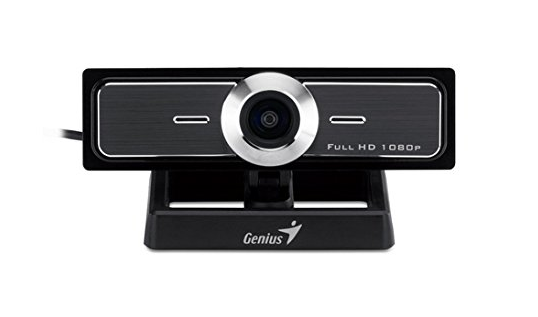
\includegraphics[width=150mm,scale=1]{./Bilder/Genius_F100_camera.png}
	\caption{Genius 120-degree Ultra Wide Angle Full HD Conference Webcam(WideCam F100) }
\end{figure}


%
\section*{3.3.Software}\label{sec:Software}
\addcontentsline{toc}{section}{3.3.Software}
%


